% =================================================================================================
% File:			mockup.tex
% Description:	Defiinisce la sezione relativa al bmockup dell'applicazione web
% Created:		2015-03-27
% Author:		Tesser Paolo
% Email:		tesser.paolo@mashup-unipd.it
% =================================================================================================
% Modification History:
% Version		Modifier Date		Change											Author
% 0.0.1 		2015-03-27 			creato scheletro								Tesser Paolo
% =================================================================================================
% 0.0.2			2015-04-13			inserite alcune descrizioni generali			Tesser Paolo
% =================================================================================================
%

% CONTENUTO DEL CAPITOLO
\appendix


\section{Mockup} % (fold)
\label{sec:mockup}
\textbf{Nota:} le immagini qui proposte sono solo un'idea iniziale di come saranno alcune pagine presenti nell'applicazione finale. Possono quindi mancare di alcuni dettagli grafici che verranno aggiunti in seguito.

	\subsection{Login} % (fold)
	\label{sub:login}
		\subsubsection{Descrizione generale} % (fold)
		La pagina di login permette all'utente, che si è già registrato al sistema, di accederci inserendo la propria email e la propria password. Se l'utente non si è ancora registrato al sistema è presente un link per effettuare la registrazione.
		% subsubsection descrizione_generale (end)

		\subsubsection{Vista desktop} % (fold)
		\begin{figure}[htbp]
			\centering
			\centerline{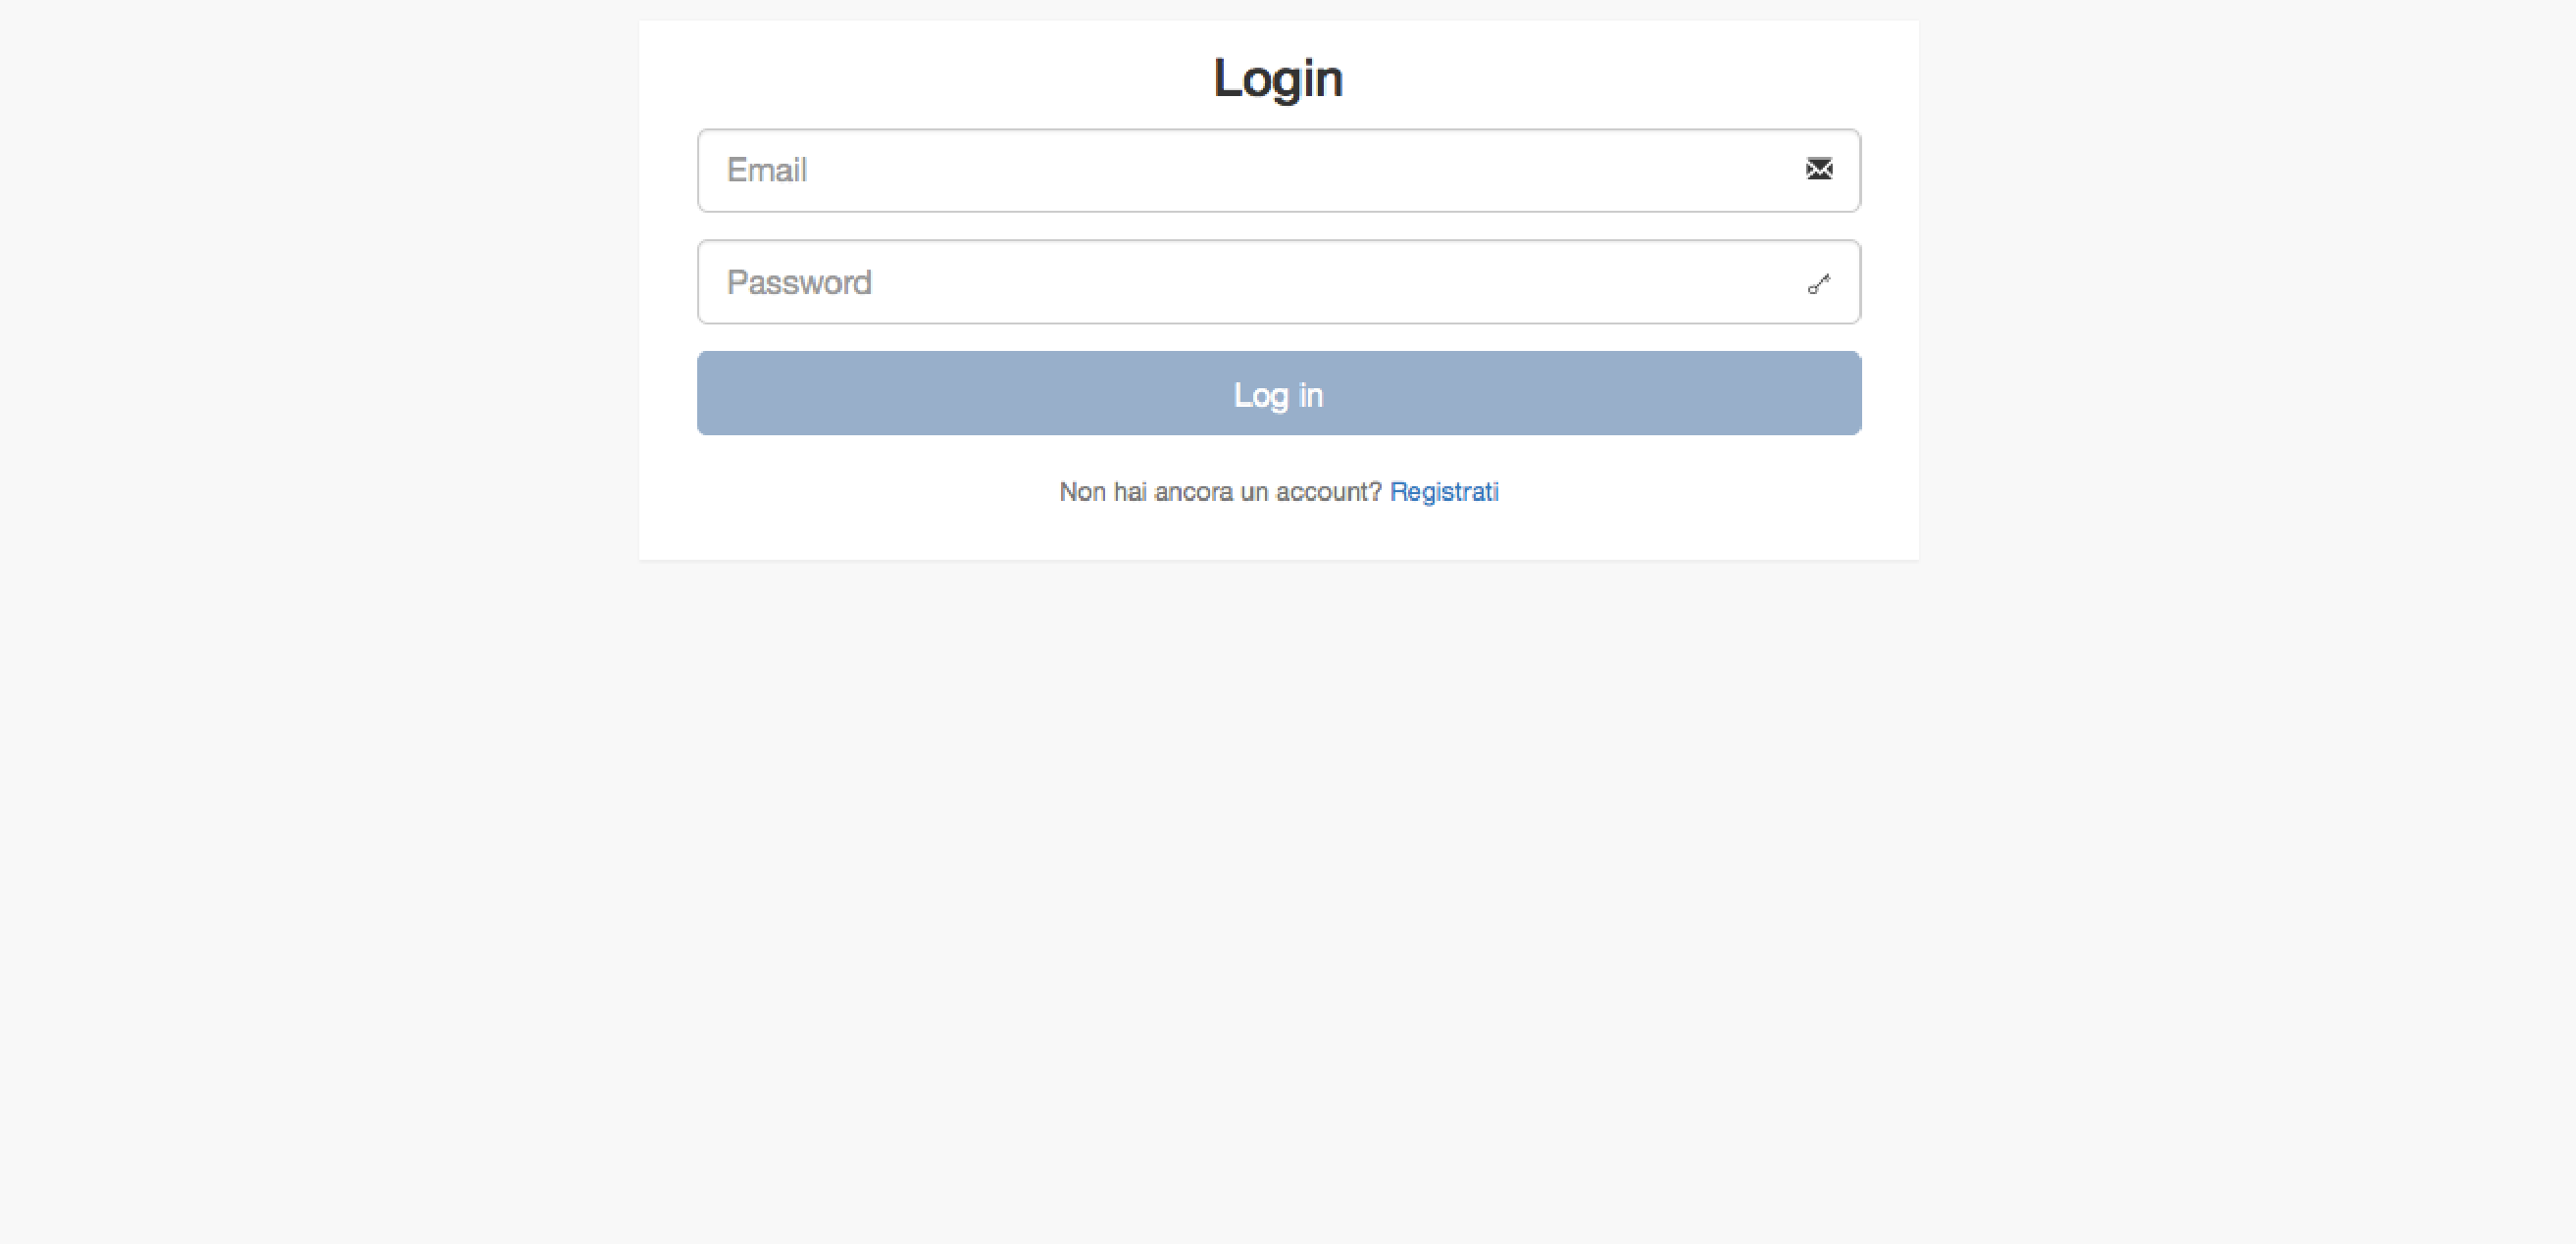
\includegraphics[scale=0.4]{./images/mockup/login_vd.pdf}}
			\caption{Page - Login (vista desktop)}
		\end{figure}
		% subsubsection vista_desktop (end)

		\subsubsection{Vista mobile} % (fold)
		\begin{figure}[htbp]
			\centering
			\centerline{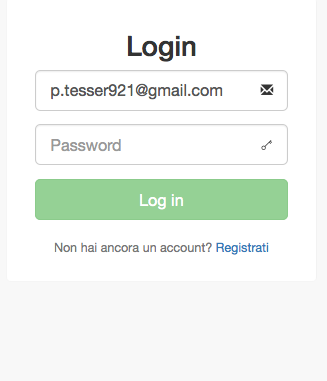
\includegraphics[scale=0.5]{./images/mockup/login_vm.png}}
			\caption{Page - Login (vista mobile)}
		\end{figure}
		% subsubsection vista_mobile (end)
	% subsection login (end)

	\subsection{Register} % (fold)
	\label{sub:register}
		\subsubsection{Descrizione generale} % (fold)
		La pagina register permette all'utente che non si è ancora registrato, di farlo, andando ad inserire uno username, una mail e una password. I campi devono essere tutti compilati e validi, altrimenti la registrazione non potrà terminare con successo.
		% subsubsection descrizione_generale (end)

		\subsubsection{Vista desktop} % (fold)
		\begin{figure}[htbp]
			\centering
			\centerline{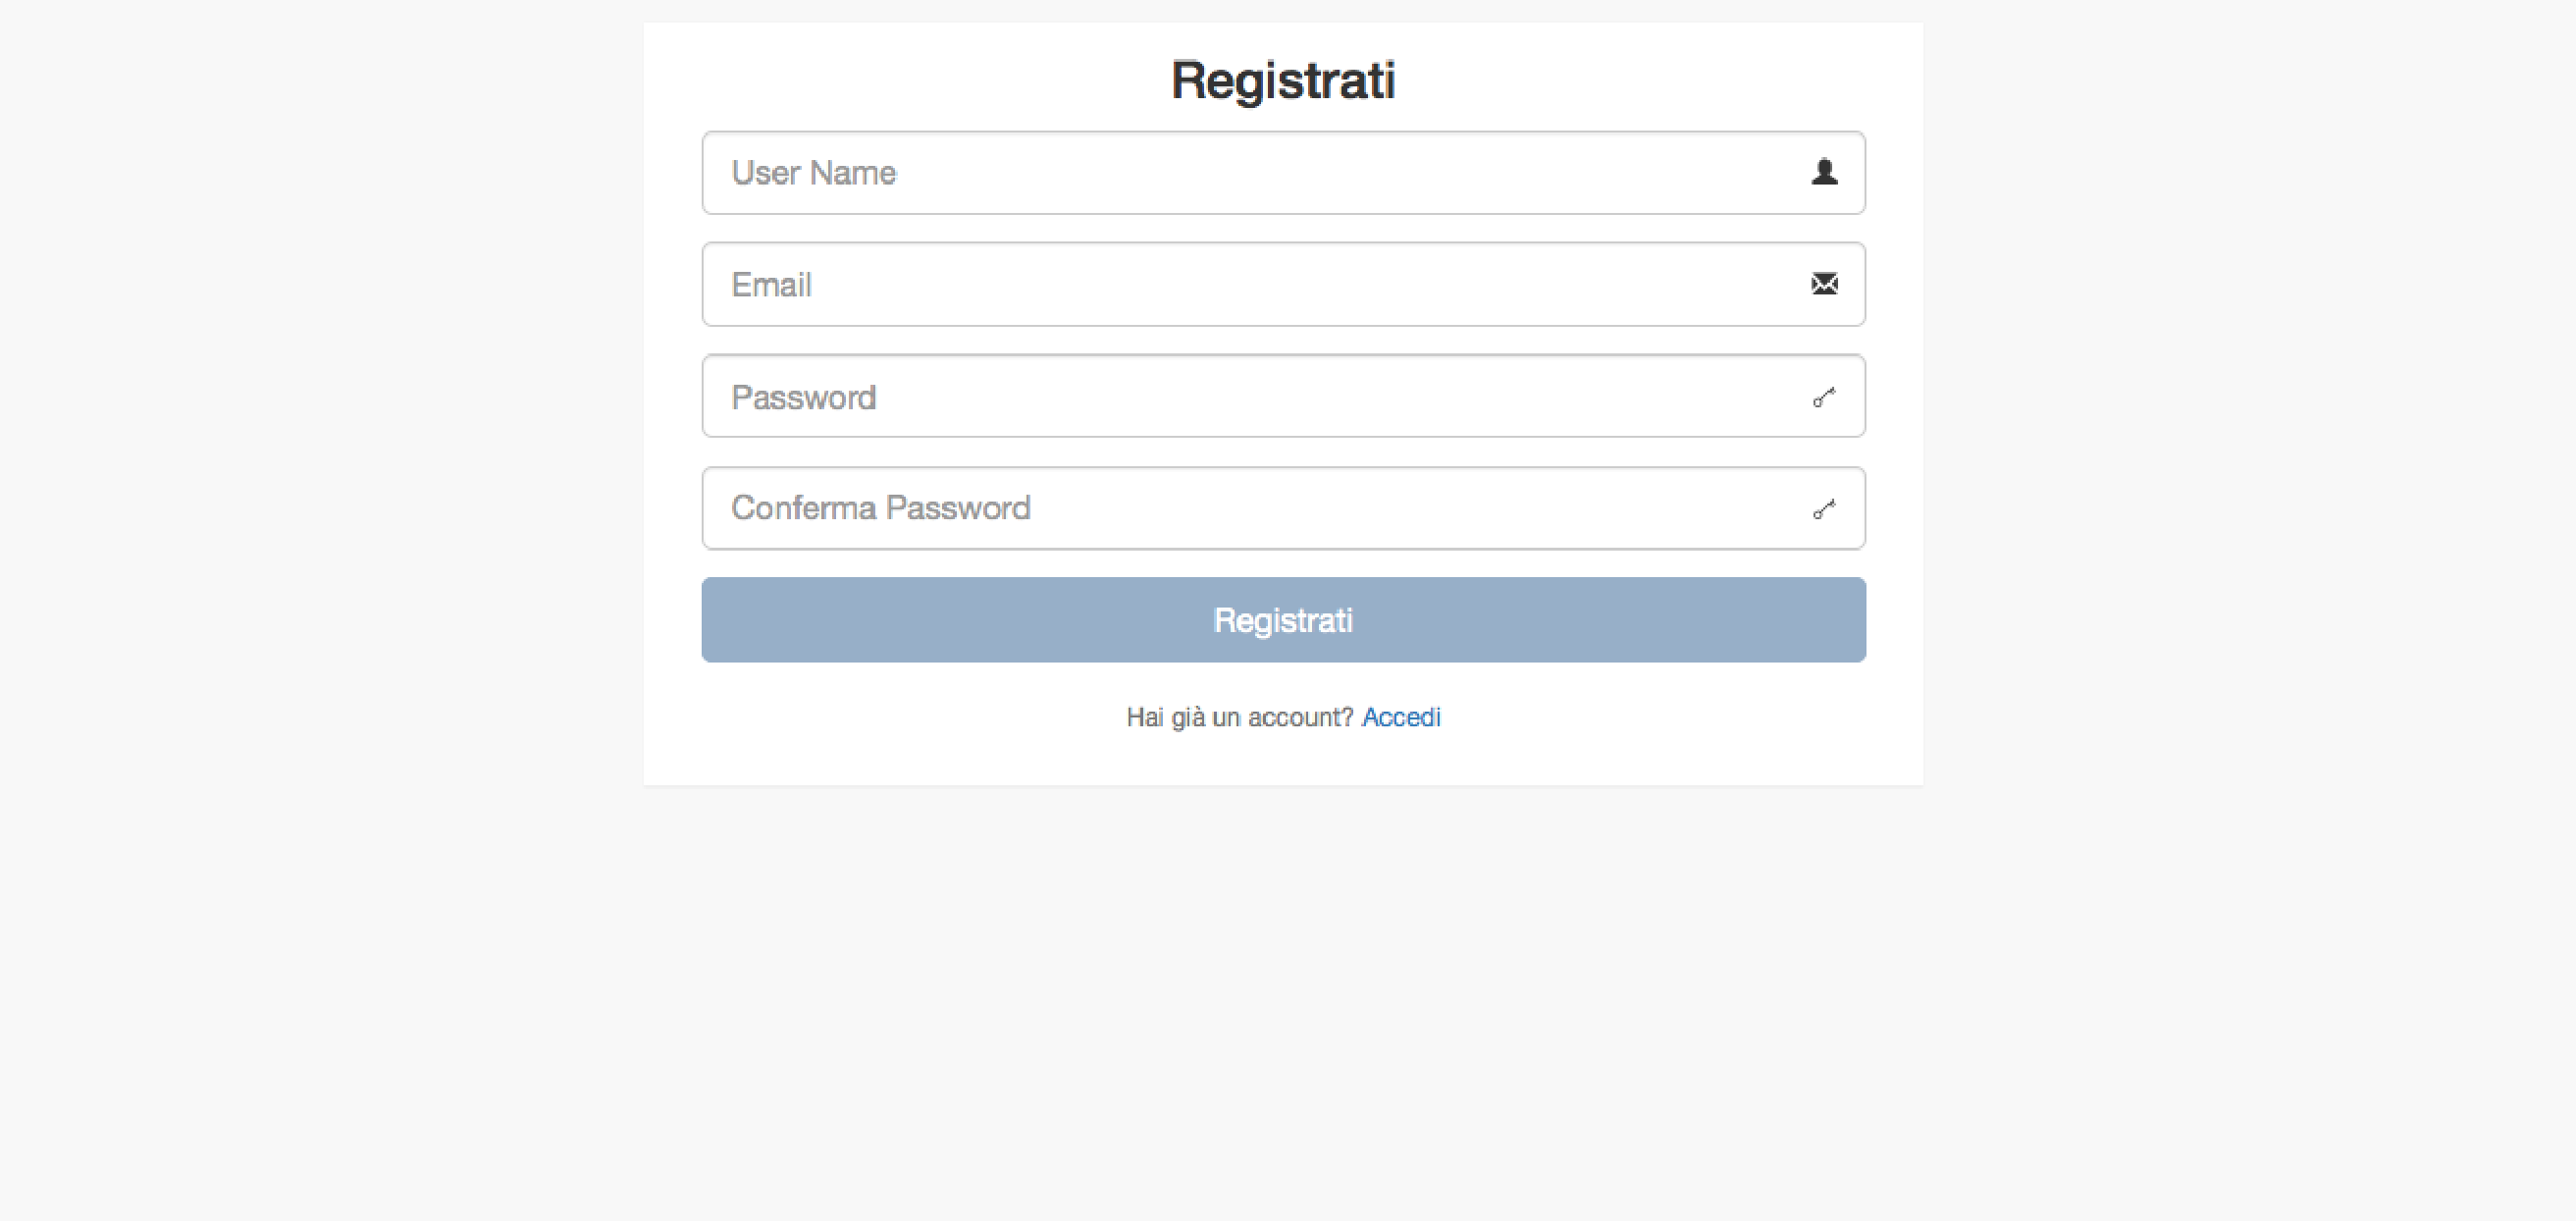
\includegraphics[scale=0.4]{./images/mockup/register_vd.pdf}}
			\caption{Page - Register (vista desktop)}
		\end{figure}
		% subsubsection vista_desktop (end)

		\subsubsection{Vista mobile} % (fold)
		\begin{figure}[htbp]
			\centering
			\centerline{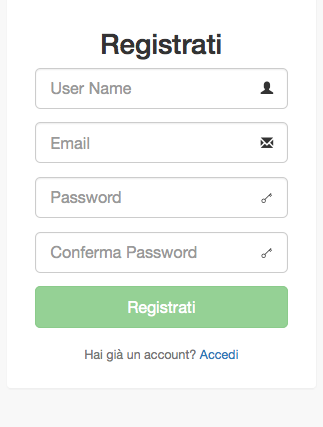
\includegraphics[scale=0.5]{./images/mockup/register_vm.png}}
			\caption{Page - Register (vista mobile)}
		\end{figure}
		% subsubsection vista_mobile (end)
	% subsection register (end)

	\subsection{Recipe} % (fold)
	\label{sub:recipe}
		\subsubsection{Descrizione generale} % (fold)
		La pagina in questione fa visualizzare tutte le recipe presenti nel sistema. Per ognuna di esse fornisce il nome e due pulsanti, uno per andare a visualizzare tutte le metriche presenti in essa e uno per andare ad effettuare un confronto tra le metriche. \newline
		\textbf{Nota}: Come informazioni generale riguardo a questa pagina e a tutte le successive si ha che da visuale desktop l'header della pagina contiene il menu principale che permette di accedere sempre alla Home page, alla pagina Settings e di effettuare il logout. Questo menu rimane invariato anche nella visuale mobile. \newline
		\'E sempre presente inoltre una barra laterale contenente i collegamenti alla pagine che incapsulano le funzionalità previste per gli utenti. Questa barra, in modalità mobile, scomparirà e verrà rimpiazzata con un menu a tendina che consentirà all'utente di avere una migliore visualizzazione del contenuto principale della pagina.
		% subsubsection descrizione_generale (end)

		\subsubsection{Vista desktop} % (fold)
		\begin{figure}[htbp]
			\centering
			\centerline{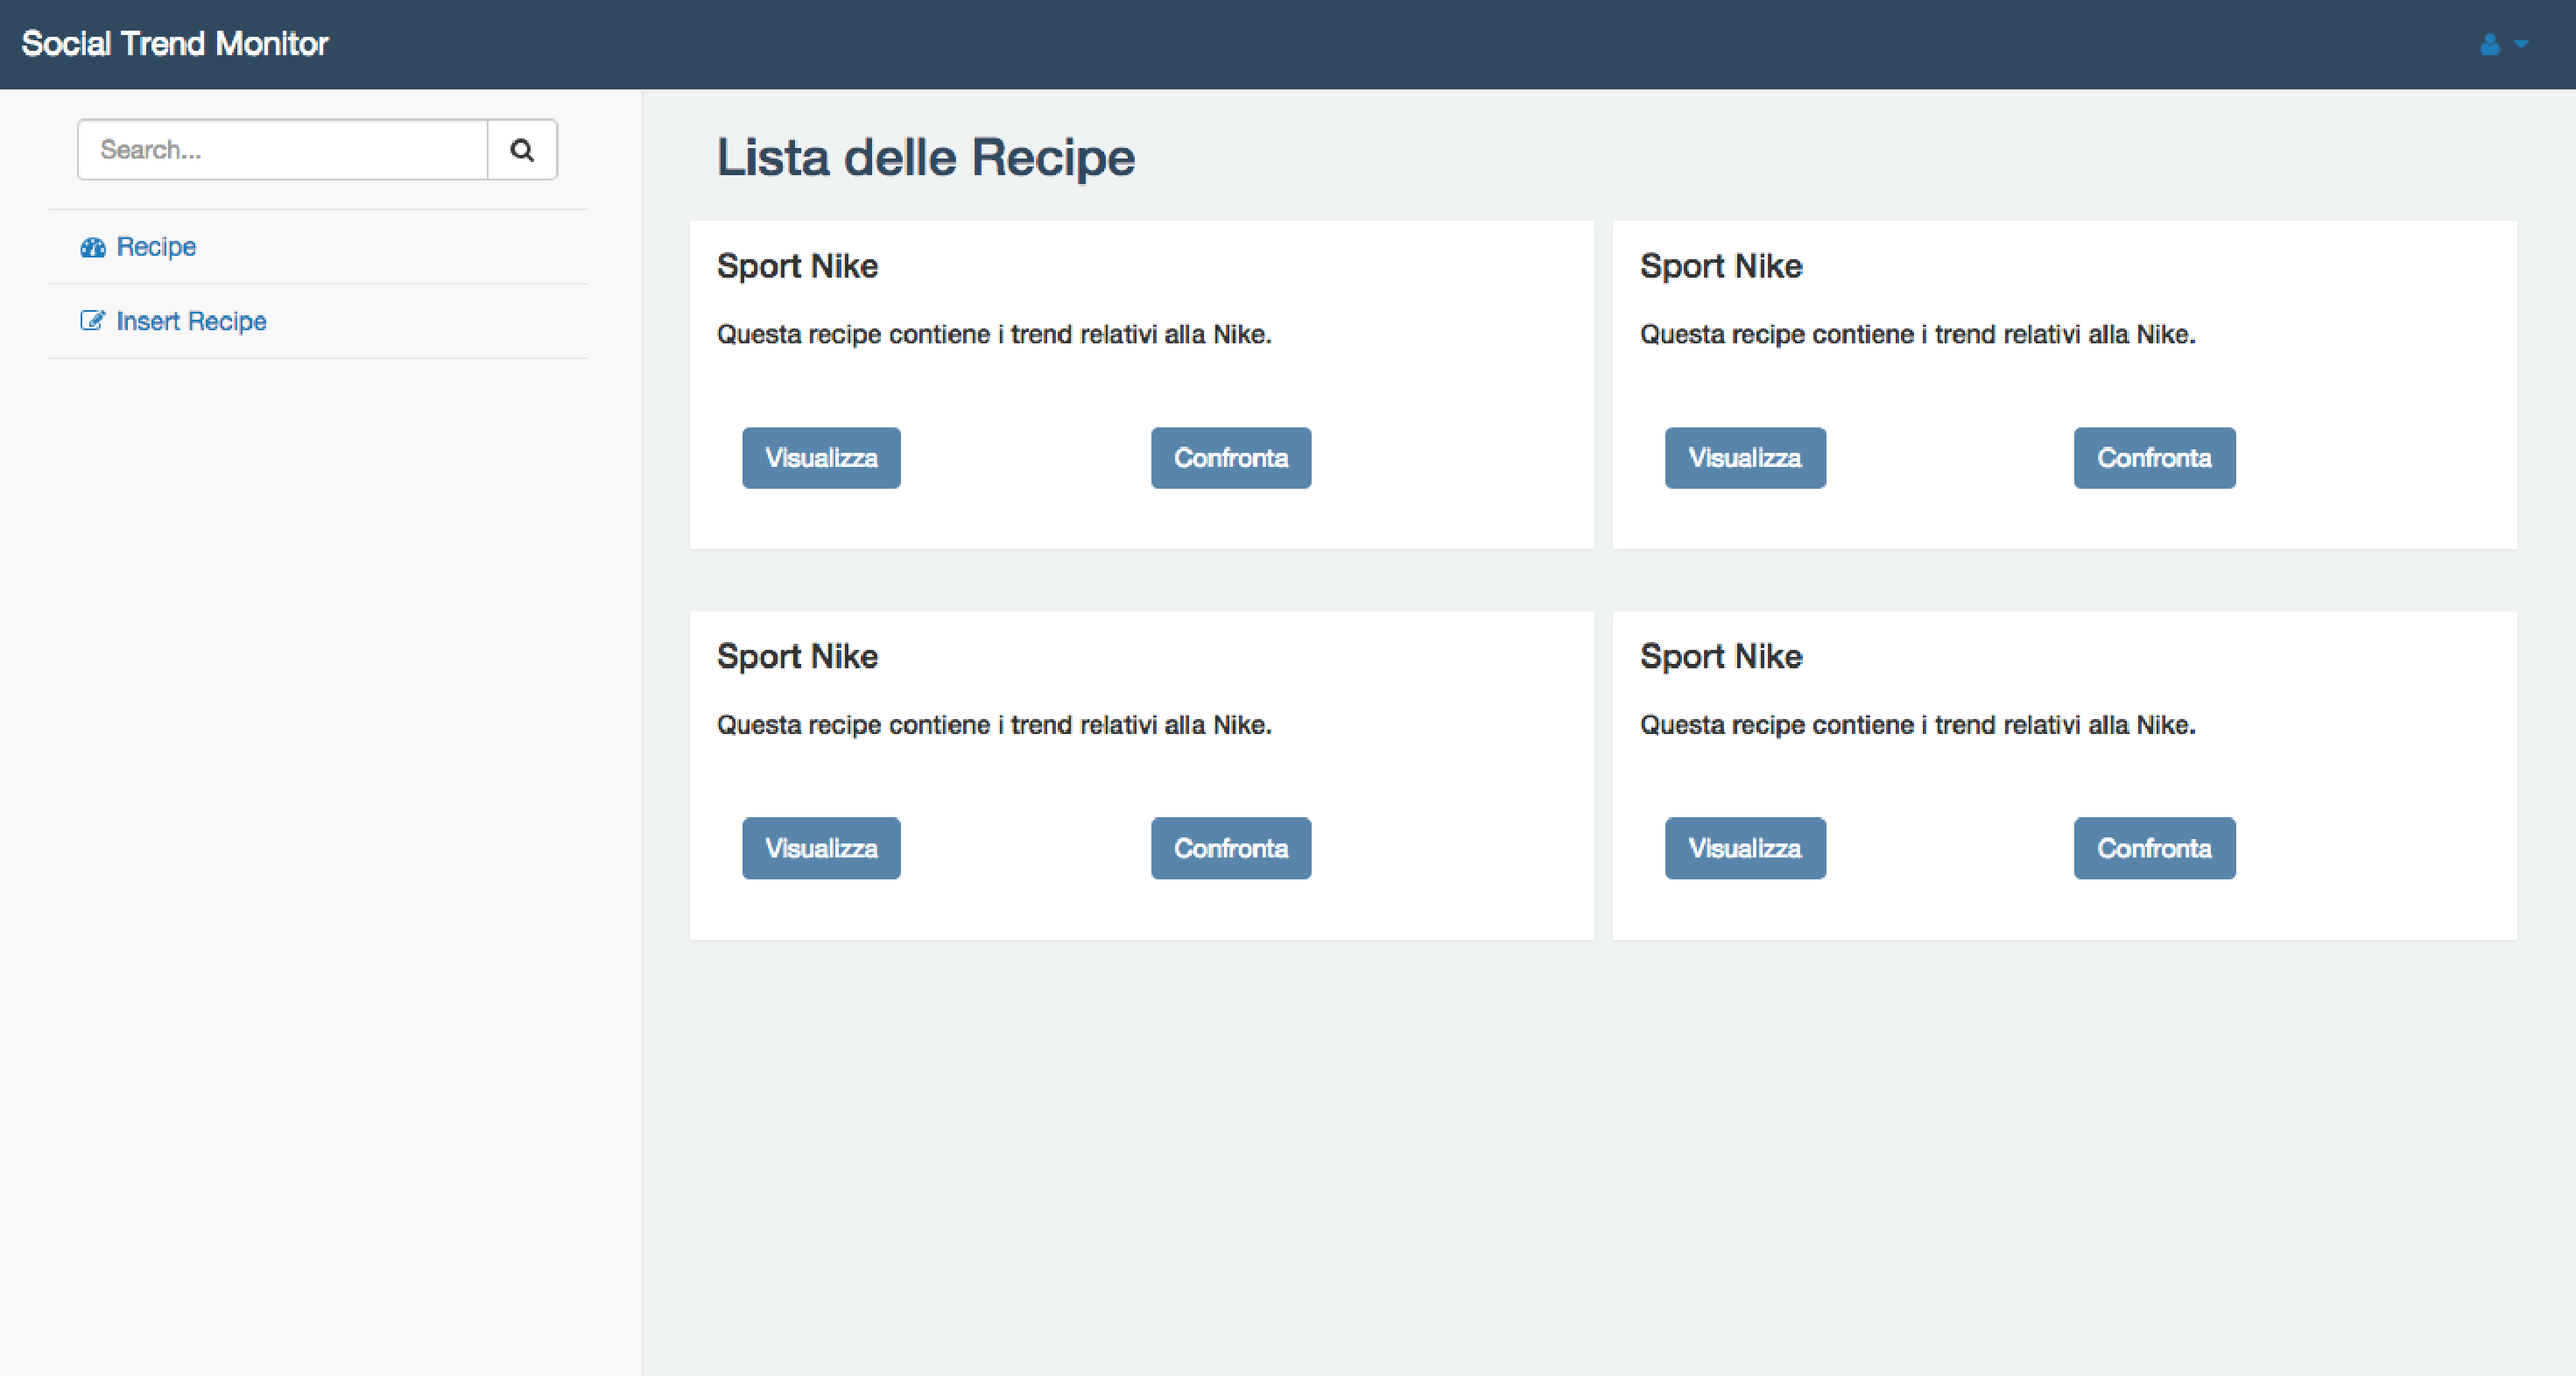
\includegraphics[scale=0.4]{./images/mockup/recipe_vd.pdf}}
			\caption{Page - Recipe (vista desktop)}
		\end{figure}
		% subsubsection vista_desktop (end)

		\subsubsection{Vista mobile} % (fold)
		\begin{figure}[htbp]
			\centering
			\centerline{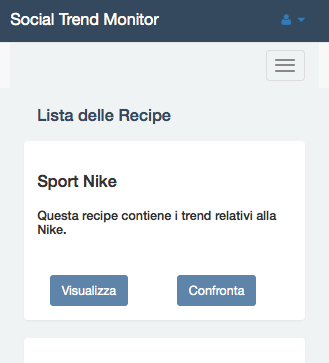
\includegraphics[scale=0.5]{./images/mockup/recipe_vm.png}}
			\caption{Page - Recipe (vista mobile)}
		\end{figure}
		% subsubsection vista_mobile (end)
	% subsection recipe (end)

	\subsection{Metrics} % (fold)
	\label{sub:metrics}
		\subsubsection{Descrizione generale} % (fold)
		La pagina metrics permette all'utente di visualizzare tutte le metriche appartenenti ad una determinata Recipe. Le metriche vengono mostrate divisi in diversi pannelli a seconda della categoria di cui fan parte.
		% subsubsection descrizione_generale (end)

		\subsubsection{Vista desktop} % (fold)
		\begin{figure}[htbp]
			\centering
			\centerline{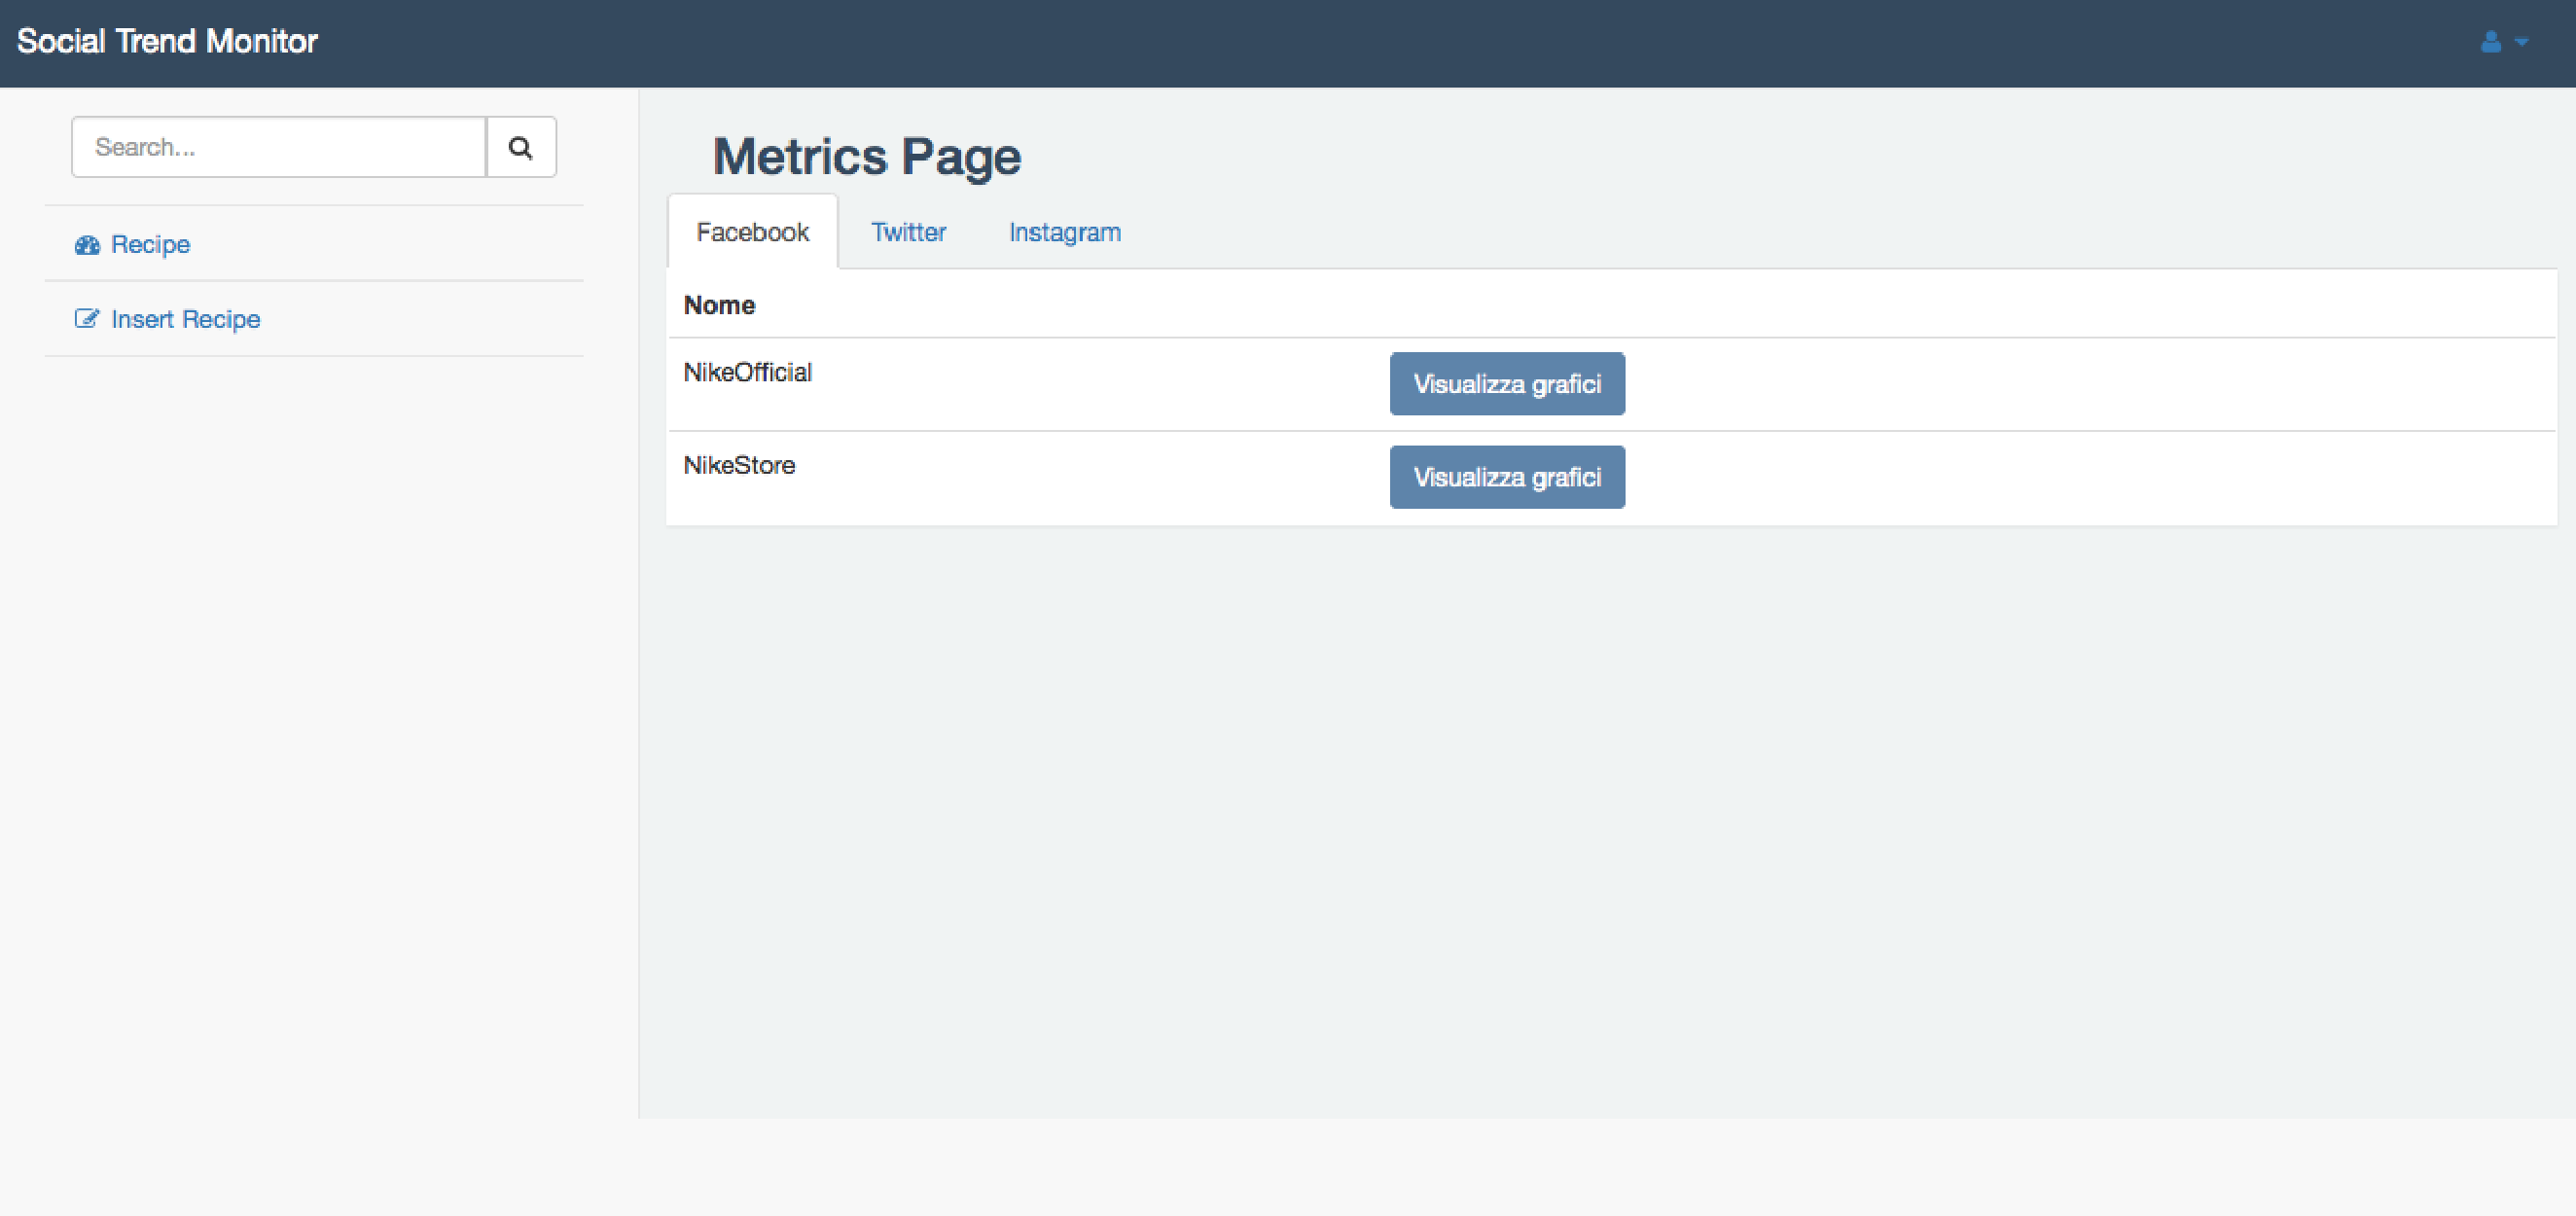
\includegraphics[scale=0.4]{./images/mockup/metrics_vd.pdf}}
			\caption{Page - Metrics (vista desktop)}
		\end{figure}
		% subsubsection vista_desktop (end)

		\subsubsection{Vista mobile} % (fold)
		\begin{figure}[htbp]
			\centering
			\centerline{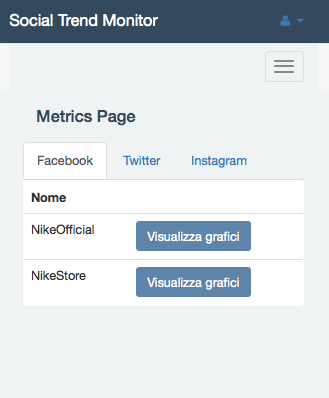
\includegraphics[scale=0.5]{./images/mockup/metrics_vm.png}}
			\caption{Page - Metrics (vista mobile)}
		\end{figure}
		% subsubsection vista_mobile (end)
	% subsubsection metrics (end)

	\subsection{Settings} % (fold)
	\label{sub:settings}
		\subsubsection{Descrizione generale} % (fold)
		La pagina settings permette all'utente di visualizzare i dati relativi al proprio account salvati nel sistema e di effettuare delle modifiche su di essi. In particolare per il cambio password, sarà richiesto di inserire la quella vecchia e successivamente per due volte quella nuova.
		% subsubsection descrizione_generale (end)

		\subsubsection{Vista desktop} % (fold)
		\begin{figure}[htbp]
			\centering
			\centerline{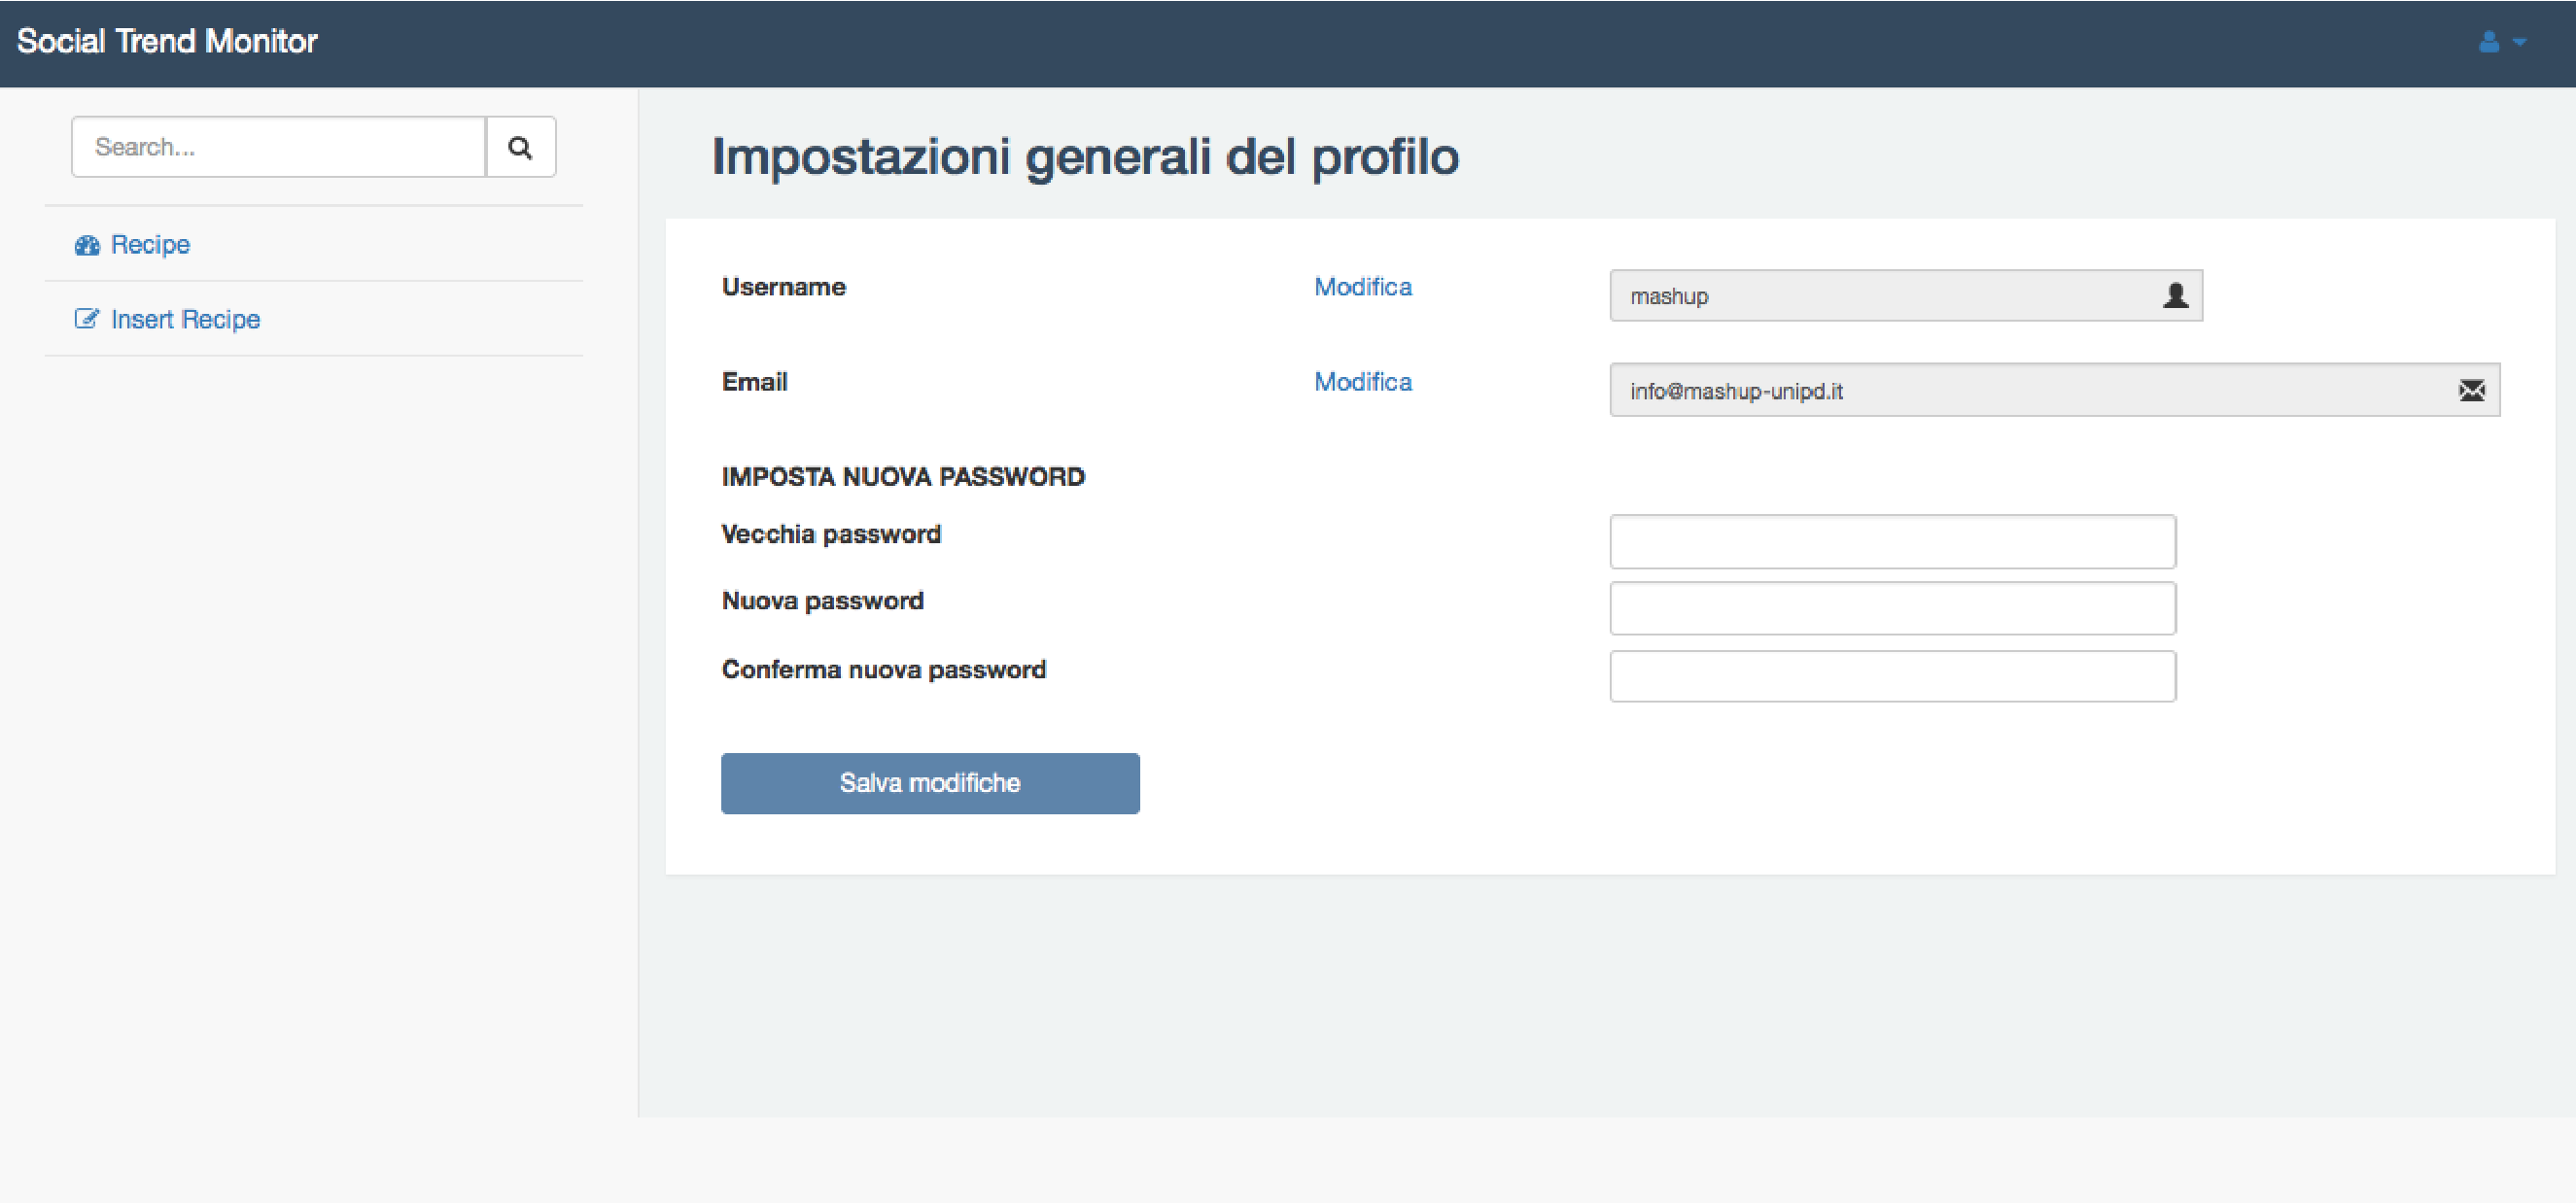
\includegraphics[scale=0.4]{./images/mockup/settings_vd.pdf}}
			\caption{Page - Settings (vista desktop)}
		\end{figure}
		% subsubsection vista_desktop (end)

		\subsubsection{Vista mobile} % (fold)
		\begin{figure}[htbp]
			\centering
			\centerline{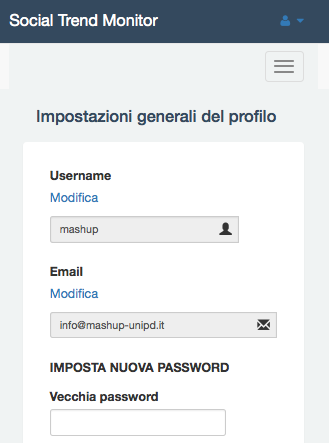
\includegraphics[scale=0.5]{./images/mockup/settings_vm.png}}
			\caption{Page - Settings (vista mobile)}
		\end{figure}
		% subsubsection vista_mobile (end)
	% subsection settings (end)

	\subsection{RecipeConfig} % (fold)
	\label{sub:recipeconfig}
		\subsubsection{Descrizione generale} % (fold)
		La pagina permette all'amministratore di andare ad inserire una nuova Recipe nel sistema. Essa visualizza un form che dovrà essere compilato in maniera adeguata per poter permettere l'inserimento della Recipe. Il form è molto guidato da scelte vincolate dal sistema tramite dei combo box che limitano i possibili errori umani. 
		% subsubsection descrizione_generale (end)

		\subsubsection{Vista desktop} % (fold)
		\begin{figure}[htbp]
			\centering
			\centerline{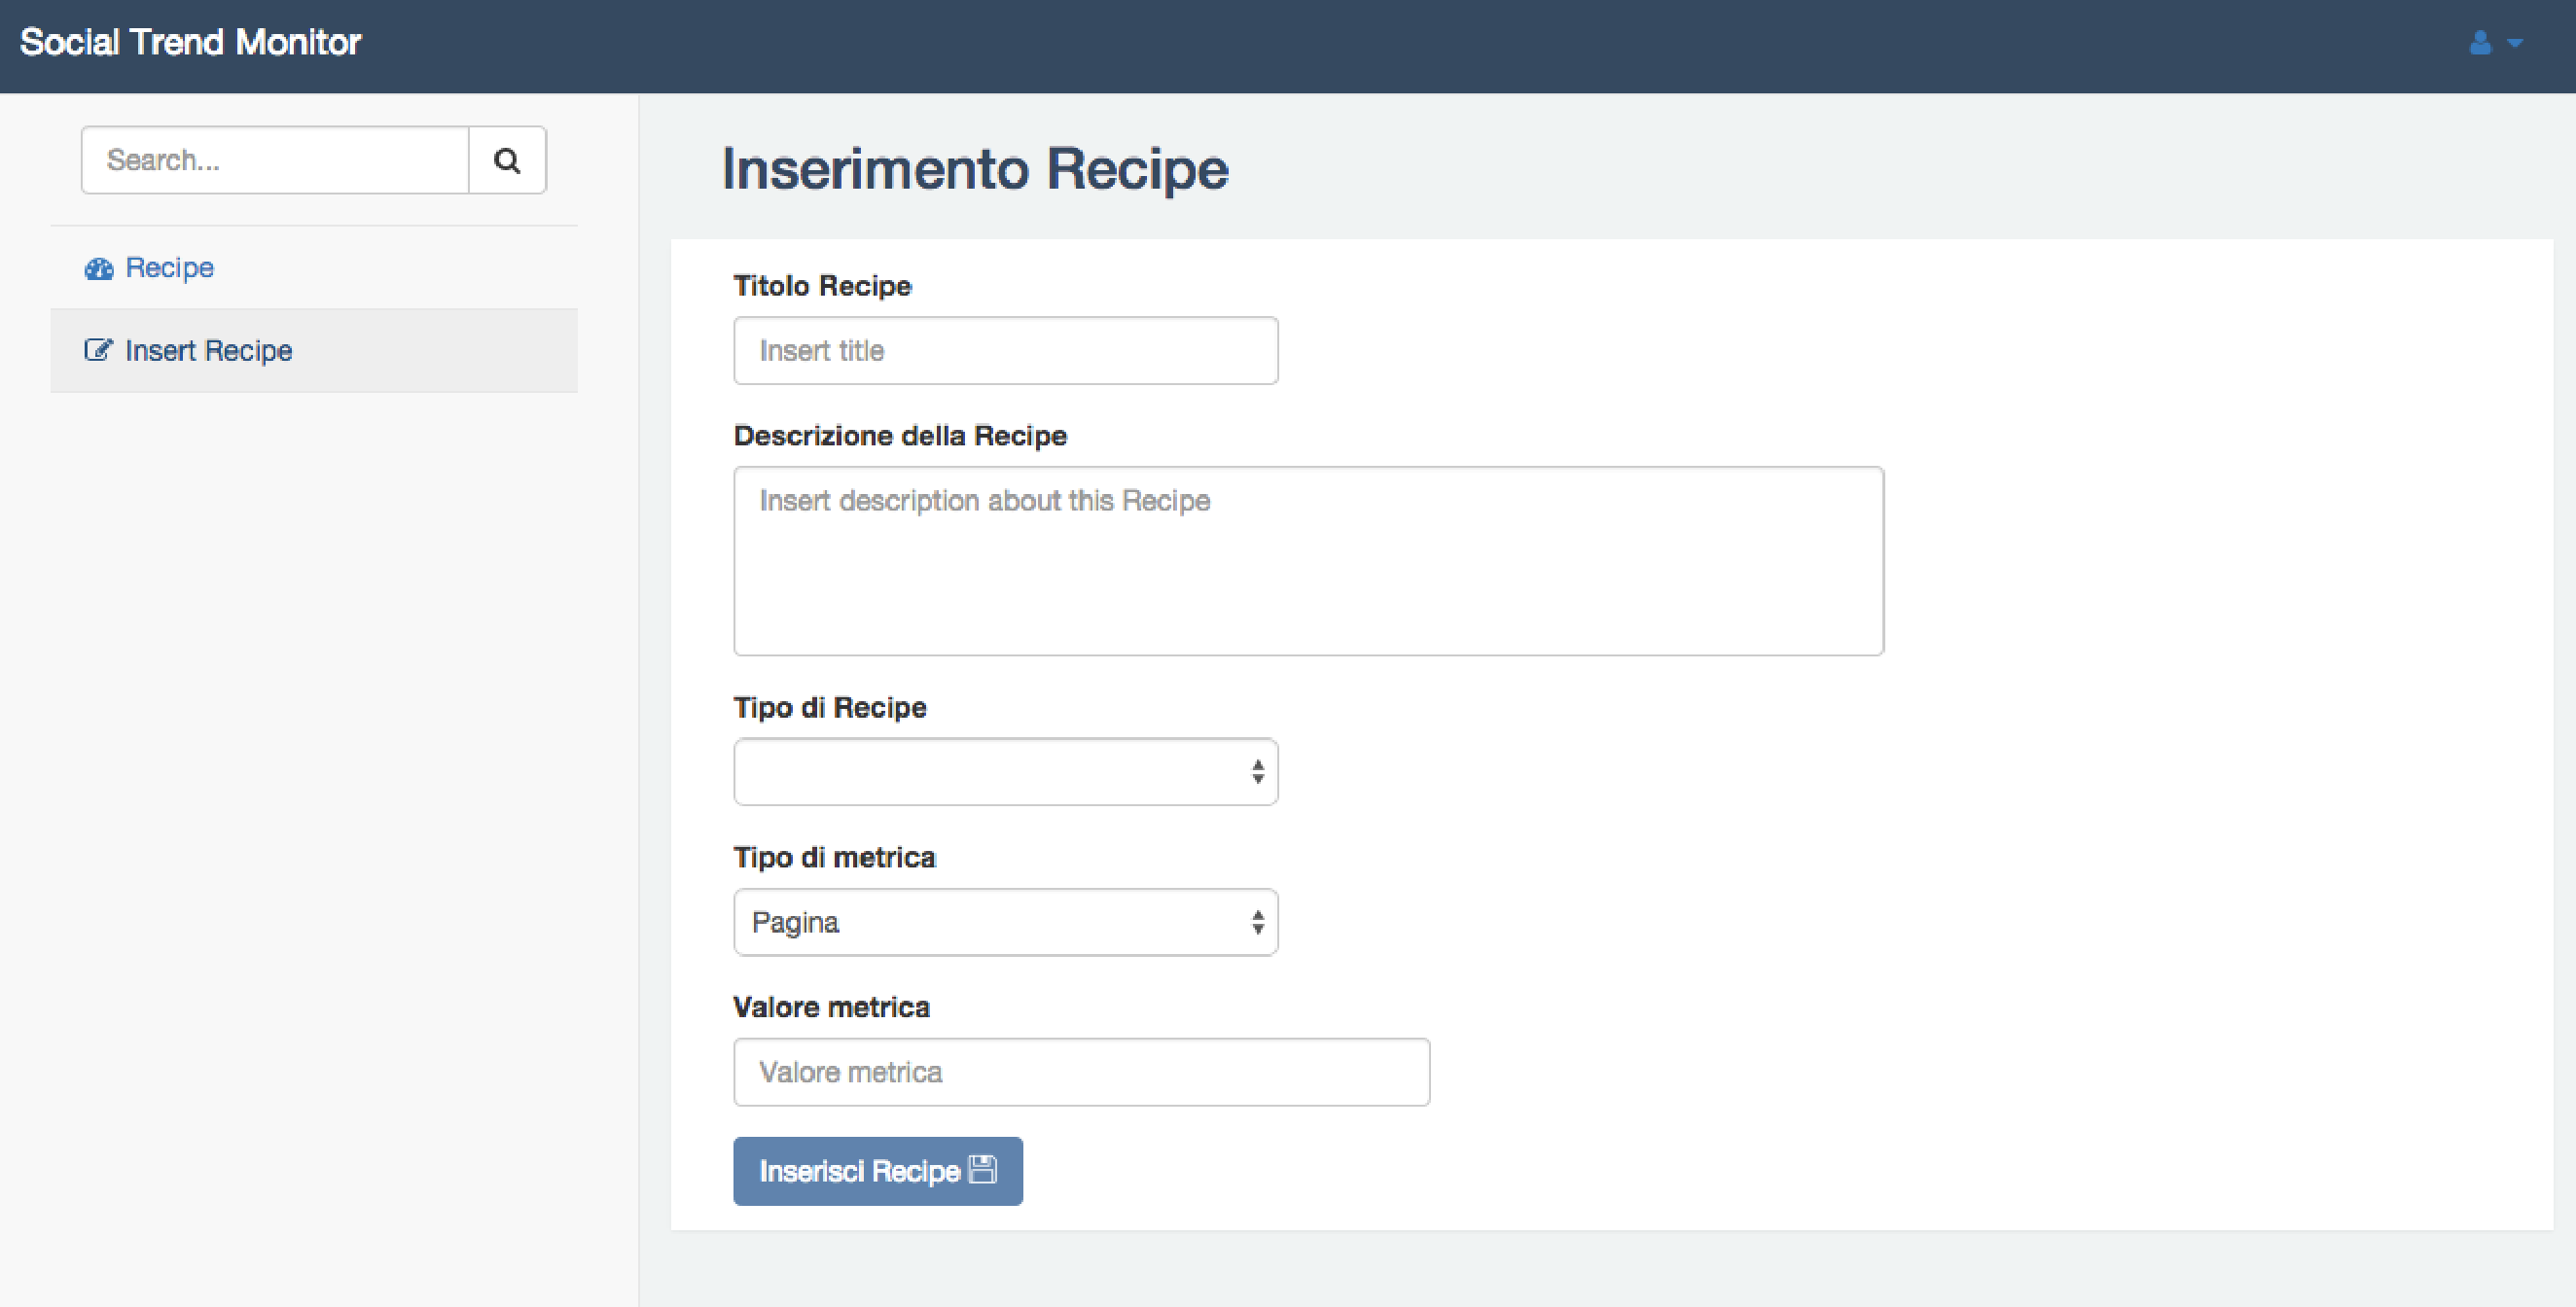
\includegraphics[scale=0.4]{./images/mockup/recipe_config_vd.pdf}}
			\caption{Page - Recipe Config (vista desktop)}
		\end{figure}
		% subsubsection vista_desktop (end)

		\subsubsection{Vista mobile} % (fold)
		\begin{figure}[htbp]
			\centering
			\centerline{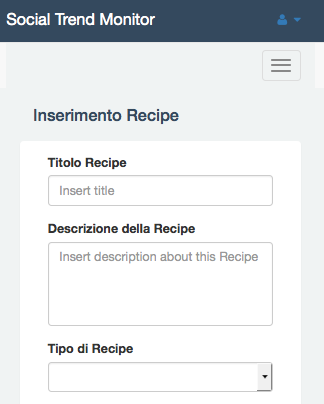
\includegraphics[scale=0.5]{./images/mockup/recipe_config_vm.png}}
			\caption{Page - Recipe Config (vista mobile)}
		\end{figure}
		% subsubsection vista_mobile (end)
	% subsubsection recipeconfig (end)


% section mockup (end)